%%
%%
\documentclass[12pt]{book}
\usepackage{amsfonts}
\usepackage{amsmath}
\usepackage{amssymb}
\usepackage{graphicx}
\usepackage{hyperref}
\usepackage{verbatim}%% \begin{comment}
\usepackage{float}%% text and image side by side
\setlength{\textheight}{10in}
\setlength{\textwidth}{7.4in}
\setlength{\topmargin}{-0.75in}
\setlength{\oddsidemargin}{-0.5in}
\setlength{\evensidemargin}{-0.5in}
\setlength{\parskip}{0.15in}
\setlength{\parindent}{0in}
\newcommand{\uvec}[1]{\boldsymbol{\hat{\text{#1}}}}%% unit vector

\newenvironment{amatrix}[1]{%
  \left(\begin{array}{@{}*{#1}{c}|c@{}}
}{%
  \end{array}\right)
}


\begin{document}


\vspace{-1.0in}\begin{center}
\Large{MCV4UR : Advanced Placement Calculus and Vectors }

\Large{Assignment \#4}


\end{center}

%\medskip

\vspace{0.015in}\hrulefill\ 

\textbf{Reference Declaration} %  Fill in your Reference Declarations in this section before your submit your assignment.

Complete the Reference Declaration section below in order for your assignment to be graded.

If you used any references beyond the course text and lectures (such as other texts, discussions with colleagues or online resources), indicate this information in the space below.  If you did not use any aids, state this in the space provided. 

Be sure to cite appropriate theorems throughout your work. You may use shorthand for well-known theorems like the MVT, IVT, etc. 

Note: Your submitted work must be \textbf{your original work}. 

Family Name: Do \\%Family Name Here
First Name: Kien %First Name Here

Declared References: \\
Reading on Math Is Fun for question 14. https://www.mathsisfun.com/algebra/matrix-inverse.html

% Type your references here.
% You can use as many lines as required.

\vspace{0.015in}\hrulefill\ 

\newpage

%%%%%%%%%%%% PROBLEMS START HERE

\begin{enumerate}

%% PROBLEM 1
\item Determine whether the following statements are True (T) or False (F).

\begin{enumerate}
\item If $\vec{u} \cdot \vec{v} = 0$ then either $\vec{u} = \vec{0}$ or $\vec{v} = \vec{0}$.\\
\textbf{False}
\item $(\vec{u} \cdot \vec{v})\vec{u} \times (\vec{u} \times \vec{v})$ is a meaningful expression.\\
\textbf{True}
\item Force and velocity are scalar quantities.\\
\textbf{False}
\item If $|\vec{a}| = 1$ then $\vec{a}$ is a unit vector.\\
\textbf{True}
\item If $\vec{a} = \vec{b} \times \vec{c}$ and $\vec{a}$ is perpendicular to both $\vec{b}$ and $\vec{c}$, then $\vec{b}$ and $\vec{c}$ are collinear.\\
\textbf{True}
\item $\left\{ \vec{i}, \left(\begin{smallmatrix} 0 \\ 1 \\ 0 \end{smallmatrix}\right), \vec{i} \times \vec{j}\right\}$ is a spanning set of $\mathbb{R}^3$.\\
\textbf{True}
\item Given the standard basis vectors $\vec{i}, \vec{j}, \vec{k} \in \mathbb{R}^3$, we can express $\vec{k}$  as a linear combination of $\vec{i}$ and $\vec{j}$.\\
\textbf{True}
\item If $\vec{a}$ and $\vec{b}$ are opposite vectors and $|\vec{a}| = n$ then $|\vec{b}| = -n$.\\
\textbf{False}
\item $\forall \vec{a}, \vec{b} \in \mathbb{R}^3$, $\vec{a} \times \vec{b} = \vec{b} \times \vec{a}$.\\
\textbf{False}
\item $\exists \vec{a}, \vec{b} \in \mathbb{R}^3$, $\vec{a} \times \vec{b} = \vec{b} \times \vec{a}$.\\
\textbf{True}
\item If $\forall m,n \in \mathbb{R}$, $|m\vec{a}| = |n\vec{a}|$ then $\vec{a}=\vec{0}$.\\
\textbf{True}

\end{enumerate}


%% I would recommend sandwiching your solution to every problem between the kind of structure I have provided below re: initial \vspace, the Solution: heading and the ending \vspace.
%\vspace{0.3cm} 
%\textbf{Solution:}\\
% Your solution starts here.
%\vspace{0.3cm}

\newpage

%% PROBLEM 2
\item Captain Picard walks 100 metres, bearing $135^{\circ}$ to reach a campsite where there are four lights. Draw a lebeled geometric vector that represents his movement in this situation.\\

\textbf{Solution:}\\
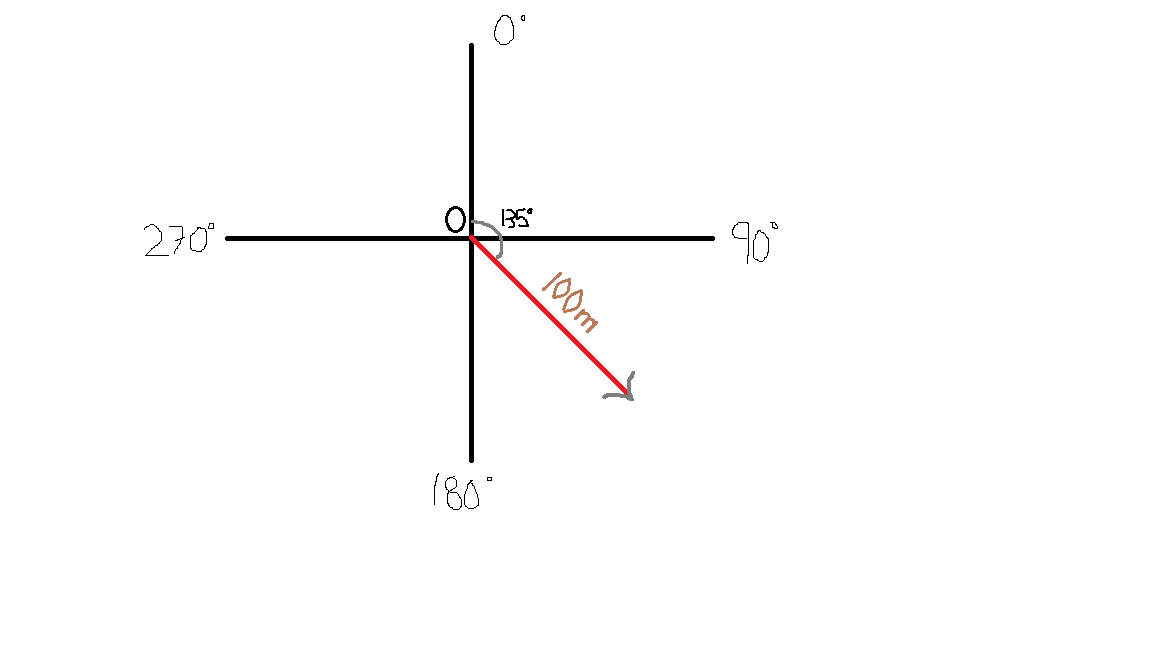
\includegraphics[scale=1]{Q2Image.png}

\newpage

%% PROBLEM 3
\setcounter{equation}{0}
\item An \textbf{orthogonal spanning set of $\mathbb{R}^3$} is a set of 3 non-zero vectors, all of which are orthogonal to each other and span $\mathbb{R}^3$. Given $\vec{a} = \left(\begin{smallmatrix} 1 \\ -1 \\ 2 \end{smallmatrix}\right)$, determine vectors $\vec{b}$ and $\vec{c}$ such that $\{\vec{a}, \vec{b}, \vec{c}\}$ is an orthogonal spanning set of $\mathbb{R}^3$. Express the vector $\vec{a}= \left(\begin{smallmatrix} 1 \\ 0 \\ 1 \end{smallmatrix}\right)$ as a linear combination of the vectors in this spanning set. \\

\textbf{Solution:}\\
Recall the dot product as well as its definition and purpose. Recall that for some $\vec{a}, \vec{b}$, if $\vec{a} \cdot \vec{b} = 0$, we have that $\vec{a}$ and $\vec{b}$ are perpendicular to each other.\\

We can start by determining $\vec{b}$ such that $\vec{a} \bot \vec{b}$ by determining the coordinates of $\vec{b}$ such that $\vec{a} \cdot \vec{b} = 0$.
\begin{align}
    0 &= \vec{a} \cdot \vec{b} \\
    0 &= (1,-1,2) \cdot (b_x, b_y, b_z) \quad \xleftarrow[]{\text{sub in given coordinates of } \vec{a}} \\
    0 &= b_x-b_y+2b_z
\end{align}
Let $b_x = 2,\; b_y = 2,\; 2b_z = 0$. Sub these values into line (3) to verify that the equation is true.
\begin{align}
    0 &\stackrel{?}{=} (2)-(2)+2(0) \\
    0 &= 0
\end{align}
Therefore, we have that $\vec{b} = (2,2,0)$ is a vector that is perpendicular to $\vec{a}$. Since $\vec{a} \bot \vec{b}$, it is also true that $\vec{a}$ and $\vec{b}$ are orthogonal to each other.\\

Now, recall the cross product and its definition. Recall that the cross product of any two vectors will yield another vector that is orthogonal to those two vectors. That is to say, for some $\vec{a} \times \vec{b} = \vec{c}$, we have that $\vec{c}$ is orthogonal to $\vec{a}$ and $\vec{b}$. So, we can simply determine $\vec{c}$ that is orthogonal to $\vec{a}$ and $\vec{b}$ by taking their cross product.
\begin{align}
    \vec{c} &= \vec{a} \times \vec{b} \\
    \vec{c} &= \begin{pmatrix}
                  \vec{i} & \vec{j} & \vec{k} \\
                  1 & -1 & 2 \\
                  2 & 2 & 0
               \end{pmatrix}\\
    \vec{c} &= (0-4)\vec{i} - (0-4)\vec{j} + (2-(-2))\vec{k} \\
    \vec{c} &= -4\vec{j} + 4\vec{j} + 4\vec{k}
\end{align}
Therefore, we have that $\vec{c} = (-4,4,4)$ is orthogonal to $\vec{a}$ and $\vec{b}$.\\

\textbf{Therefore, $\{\vec{a}, \vec{b}, \vec{c}\}$ is an orthogonal spanning set of $\mathbb{R}^3$ for $\vec{a} = \left(\begin{smallmatrix} 1 \\ -1 \\ 2 \end{smallmatrix}\right)$, $\vec{b} = \left(\begin{smallmatrix} 2 \\ 2 \\ 0 \end{smallmatrix}\right)$ and $\vec{c} = \left(\begin{smallmatrix} -4 \\ 4 \\ 4 \end{smallmatrix}\right)$}. \\

\newpage
%% Question 3 part 2
\textbf{Express the vector $\vec{v}= \left(\begin{smallmatrix} 1 \\ 0 \\ 1 \end{smallmatrix}\right)$ as a linear combination of the vectors in this spanning set.}\\
We have $\vec{v}= \left(\begin{smallmatrix} 1 \\ 0 \\ 1 \end{smallmatrix}\right)$, $\vec{a} = \left(\begin{smallmatrix} 1 \\ -1 \\ 2 \end{smallmatrix}\right)$, $\vec{b} = \left(\begin{smallmatrix} 2 \\ 2 \\ 0 \end{smallmatrix}\right)$ and $\vec{c} = \left(\begin{smallmatrix} -4 \\ 4 \\ 4 \end{smallmatrix}\right)$.\\

Consider $p,q,r \in \mathbb{R}$ such that $\vec{v} = p\vec{a}+q\vec{b}+r\vec{z}$. Solve for $p,q,r$ by creating an augmented matrix and reducing it into Row Echelon Form(REF). \\
\begingroup
\addtolength{\jot}{0.5em}
\begin{align}
    &\begin{amatrix}{3}
       1 & 2 & -4 & 1 \\
       -1 & 2 & 4 & 0 \\
       2 & 0 & 4 & 1 
    \end{amatrix}\\
    \equiv
    \substack{{R_2}^{'} = R_1+R_2 \\
    {R_3}^{'} = 2R_1-R_3}
    &\begin{amatrix}{3}
       1 & 2 & -4 & 1 \\
       0 & 4 & 0 & 1 \\
       0 & 4 & -12 & 1 
    \end{amatrix}\\
    \equiv
    \substack{ \\
    R_3^{'} = R_2-R_3}
    &\begin{amatrix}{3}
       1 & 2 & -4 & 1 \\
       0 & 4 & 0 & 1 \\
       0 & 0 & 12 & 0 
    \end{amatrix}
\end{align}
\endgroup
Now that the augmented matrix is in REF, we can now solve for $p,q,r$.\\
Solve for $r$,
\begin{align}
    0 &= 12 r \\
    r &= 0
\end{align}
Solve for $q$,
\begin{align}
    1 &= 4q \\
    q &= \dfrac{1}{4}
\end{align}
Solve for $p$,
\begin{align}
    1 &= 1p+2q-4r \\
    p &= 1+4r-2q \\
    p &= 1+4(0)-2\left(\dfrac{1}{4}\right) \\
    p &= \dfrac{1}{2}
\end{align}
So, we have that
$$\vec{v} = \dfrac{1}{2}\vec{a} + \dfrac{1}{4}\vec{b}$$

%% begin comment
\begin{comment}
    \begin{equation}
        \begin{cases}
                1 &= p+q+3r\\
                0 &= -p-q+3r\\
                1 &= 2p-q+0r
        \end{cases}
    \end{equation}
    We can see that by adding the first(top) and second(middle) equation in line (10), we get the following,\\
    \begin{equation}
        +\begin{cases}
                1 &= p+q+3r\\
                0 &= -p-q+3r\\
                \hline
                1 &= 6r\\
        \end{cases}
    \end{equation}
    $$r = \dfrac{1}{6}$$
    Now, looking back at line (10), let's add the first(top) and third(bottom) equation together. We have,\\
    \begin{equation}
        +\begin{cases}
                1 &= p+q+3r\\
                1 &= 2p-q+0r\\
                \hline
                2 &= 3p + 3r\\
        \end{cases}
    \end{equation}
    Rearrange line (12) then sub in $r=\dfrac{1}{6}$ which we determined from line (11) and solve for $p$.
    \begin{align}
        2 &= 3p + 3r \\
        p &= \dfrac{2-3r}{3} \\
        p &= \dfrac{2-3\left(\frac{1}{6}\right)}{3} \\
        p &= \dfrac{1}{2}
    \end{align}
    Finally, determine $q$ by subbing in $p=\dfrac{1}{2}$ into the third equation in line (10).
    \begin{align}
        1 &= 2p-q\\
        q &= 2p-1\\
        q &= 2\left(\dfrac{1}{2}\right)-1\\
        q &= 0
    \end{align}
    Finally, we have that $p = \dfrac{1}{2}, q = 0, r = \dfrac{1}{6}$.\\
\end{comment}
%% end comment

\textbf{Therefore, we have that $\vec{v}= \left(\begin{smallmatrix} 1 \\ 0 \\ 1 \end{smallmatrix}\right)$ as a linear combination of the vectors in this spanning set is $\left(\begin{smallmatrix} \frac{1}{2} \\ \frac{1}{4} \\ 0 \end{smallmatrix}\right)$}

\newpage

%% PROBLEM 4
\item Verify \emph{Lagrange's Identity}, $|\vec{u} \times \vec{v}|^2 = |\vec{u}|^2|\vec{v}|^2 - (\vec{u} \cdot \vec{v})^2$, for $\vec{u} = \left(\begin{smallmatrix} 0 \\ 3 \\ 4 \end{smallmatrix}\right)$ and $\vec{v}= \left(\begin{smallmatrix} 4 \\ 0 \\ 3 \end{smallmatrix}\right)$.\\

\textbf{Solution:}\\
\setcounter{equation}{0}
Solve the left side and the right side separately and if both sides yield the same outcome, Lagrange's Identity would be verified.

Let's begin with the left side, we have,
\begin{align}
    &= |\vec{u} \times \vec{v}|^2 \\
    &= \left[(0,3,6) \times (4,0,3)\right]^2 \xleftarrow[]{\text{sub in given values of } \vec{u} \text{ and } \vec{v}}
\end{align}
Evaluate $\vec{u} \times \vec{v}$ or $\left(\begin{smallmatrix} 0 \\ 3 \\ 4\end{smallmatrix}\right) \times \left(\begin{smallmatrix} 4 \\ 0 \\ 3 \end{smallmatrix}\right)$ separately,
\begingroup
\addtolength{\jot}{0.5em}
\begin{align}
    &= \vec{u} \times \vec{v} \\
    &= \begin{pmatrix}
          \vec{i} & \vec{j} & \vec{k} \\ 
          0 & 3 & 4 \\
          4 & 0 & 3
       \end{pmatrix}\\
    &= 9\vec{i} + 16\vec{j} - 12\vec{k} \\
    &= (9,16,-12)
\end{align}
\endgroup
Sub $(9,16,-12)$ from line (6) into line (2) to continue solving the left side,
\begin{align}
    &= |(9,16,-12)|^2 \\
    &= \left( \sqrt{9^2+16^2+(-12)^2} \right)^2 \\
    &= \sqrt{481}^2 \\
    &= 481
\end{align}
Now, let's evaluate the right side of the equation,
\begin{align}
    &= |\vec{u}|^2|\vec{v}|^2 - (\vec{u} \cdot \vec{v})^2 \\
    &= \sqrt{(0^2+3^2+4^2)}^2 \sqrt{(4^2+0^2+3^2)}^2 - \left[(0,3,4)\cdot(4,0,3)\right] \\
    &= (0^2+3^2+4^2)(4^2+0^2+3^2) - \left[(0,3,4)\cdot(4,0,3)\right]\\
    &= 625 - 12^2 \\
    &= 625 - 144 \\
    &= 481
\end{align}
\textbf{Since the left side of the equation equals 481 and the right side of the equation also equals 481, both sides yield the same value therefore Lagrange's Identity is verified.}

\newpage

%% PROBLEM 5
\item Consider non-zero vectors $\vec{a}, \vec{b}, \vec{c} \in \mathbb{R}^2$ such that $\vec{b}$ and $\vec{c}$ are collinear.
%% =======  a  ========
\begin{enumerate}
\item Sketch a possible graphical representation of $proj_{\vec{b}}\vec{a}$ and $proj_{\vec{c}}\vec{a}$.\\

\textbf{Solution:}\\
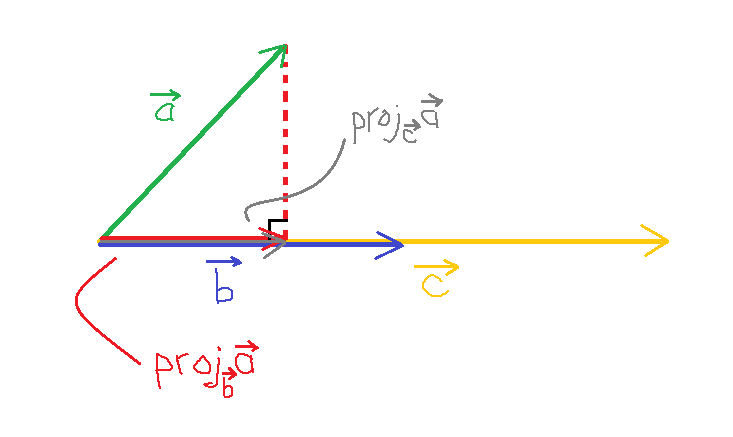
\includegraphics[scale=0.8]{Q5aImage(1).png}

%% =======  PROBLEM 5b  ========

\item Prove $proj_{\vec{b}}\vec{a} = proj_{\vec{c}}\vec{a}$.\\

\textbf{Solution:}\\
Recall that $$proj_{\vec{b}}\vec{a} = \dfrac{\vec{a} \cdot \vec{b}}{|\vec{b}|^2} \, \vec{b}$$
Also, recall Theorem 3.2 (pg. 714) states that for some angle $\theta$ between nonzero $\vec{a}$ and $\vec{b}$. Then,
$$\vec{a} \cdot \vec{b} = |\vec{a}||\vec{b}|\cos\theta$$
Combining these two theorems, we have,
\setcounter{equation}{0}
\begingroup
\addtolength{\jot}{0.5em}
\begin{align}
    proj_{\vec{b}}\vec{a} &= \dfrac{\vec{a} \cdot \vec{b}}{|\vec{b}|^2} \, \vec{b} \\
    proj_{\vec{b}}\vec{a} &= \dfrac{|\vec{a}||\vec{b}|\cos\theta}{|\vec{b}|^2} \, \vec{b} \qquad \qquad \xleftarrow[]{\vec{a} \cdot \vec{b} \,=\, |\vec{a}||\vec{b}|\cos\theta}\\
    proj_{\vec{b}}\vec{a} &= \dfrac{|\vec{a}|\cos\theta}{|\vec{b}|} \, \vec{b}
\end{align}
\endgroup
Recall that $\dfrac{\vec{b}}{|\vec{b}|}$ represents a unit vector in the direction of $\vec{b}$. Therefore, we can rewrite line (3) as follows,
\begingroup
\addtolength{\jot}{0.5em}
\begin{align}
    proj_{\vec{b}}\vec{a} &= |\vec{a}|\cos\theta \, \dfrac{\vec{b}}{|\vec{b}|} \\
    proj_{\vec{b}}\vec{a} &= |\vec{a}| \cos\theta \, \hat{b}
\end{align}
\endgroup

By the same token, we can perform the same process for $proj_{\vec{c}}\vec{a}$.
\begingroup
\addtolength{\jot}{0.5em}
\begin{align}
    proj_{\vec{c}}\vec{a} &= \dfrac{\vec{a} \cdot \vec{c}}{|\vec{c}|^2} \, \vec{c} \\
    proj_{\vec{c}}\vec{a} &= \dfrac{|\vec{a}||\vec{c}|\cos\theta}{|\vec{c}|^2} \, \vec{c} \qquad \qquad \xleftarrow[]{\vec{a} \cdot \vec{c} \,=\, |\vec{a}||\vec{c}|\cos\theta}\\
    proj_{\vec{c}}\vec{a} &= \dfrac{|\vec{a}|\cos\theta}{|\vec{c}|} \, \vec{c} \\
    proj_{\vec{c}}\vec{a} &= |\vec{a}|\cos\theta \, \dfrac{\vec{c}}{|\vec{c}|} \\
    proj_{\vec{c}}\vec{a} &= |\vec{a}| \cos\theta \, \hat{c}
\end{align}
\endgroup

Since $\vec{a}$ and $\vec{b}$ are collinear, we know that they are parallel to each other. In terms of direction, we have two cases: both projection vectors point in the same direction, the projections vectors point in opposite directions. Consider and prove $proj_{\vec{b}}\vec{a} = proj_{\vec{c}}\vec{a}$ in each case, separately.\\

\textbf{Case 1: Projection vectors point in the same direction}\\
Since $\vec{b}$ and $\vec{c}$ are collinear and point in the same direction, their normal vectors must also point in the same direction. Recall that the normal vector of any vector is just that vector with a magnitude of one. Since $\vec{a}$ and $\vec{b}$ are collinear, we have that their normal vectors are equivalent in magnitude and direction. Therefore, we can say that,
$$\hat{b} = \hat{c}$$
from line (5) and line (10). Since $\hat{b} = \hat{c}$, we can also say that,
$$|\vec{a}| \cos\theta \, \hat{b} = |\vec{a}| \cos\theta \, \hat{c}$$
And since $proj_{\vec{b}}\vec{a} = |\vec{a}| \cos\theta \, \hat{b}$ and $proj_{\vec{c}}\vec{a} = |\vec{a}| \cos\theta \, \hat{c}$, it is true that
$$proj_{\vec{b}}\vec{a} = proj_{\vec{c}}\vec{a}$$

\textbf{Case 2: Projection vectors point in opposite directions}\\
Earlier, we mentioned that $\hat{b}$ and $\hat{c}$ are of equal magnitude. Since $\vec{b}$ and $\vec{c}$ point in opposite directions, we can say that,
$$\hat{b} = -\hat{c}$$
Since $\hat{b}$ and $\hat{c}$ are parallel and point in opposite directions, if we place the initial points of $\hat{b}$ and $\hat{c}$ together, we effectively have created a $180^{\circ}$. We have that the cosine of angle $\theta$ created by $\hat{b}$ will equal the negative cosine of the angle $\gamma$ created by $\hat{c}$. Therefore, we have that,
\begin{align}
    |\vec{a}| \cos\theta \, \hat{b} = |\vec{a}| (-\cos\theta) \, (-\hat{c}) \\
    |\vec{a}| \cos\theta \, \hat{b} = |\vec{a}| \cos\theta \, \hat{c}\\
    proj_{\vec{b}}\vec{a} = proj_{\vec{c}}\vec{a}
\end{align}
\textbf{Therefore, regardless of the direction and magnitude of $\vec{a}, \vec{b}$ and $\vec{c}$, as long as $\vec{b}$ and $\vec{c}$ are collinear, we have that
$$proj_{\vec{b}}\vec{a} = proj_{\vec{c}}\vec{a}$$}



\item Explain \emph{briefly} in words why $proj_{\vec{b}}\vec{a} = proj_{\vec{c}}\vec{a}$.\\

\textbf{Solution:}\\
Since $\vec{b}$ and $\vec{c}$ are collinear, $\vec{b}$ and $\vec{c}$ are parallel and can either: go in the same direction or go in opposite directions. I will explain each case separately starting with the first case.\\

\textbf{Case 1: $\vec{b}$ and $\vec{c}$ point in the same direction}\\
Refer back to the figure in part (a), we can see that $proj_{\vec{b}}\vec{a}$ and $proj_{\vec{c}}\vec{a}$ depend on the magnitude of $\vec{a}$ and the angle created between $\vec{a}$ and $\vec{b}$, $\vec{a}$ and $\vec{c}$, respectively, but does not depend on the magnitude of $\vec{b}$ nor $\vec{c}$. We can also see that
the magnitude of $proj_{\vec{b}}\vec{a} = proj_{\vec{c}}\vec{a}$.\\

Since the $\vec{b}$ and $\vec{c}$ are collinear, we have that the angle between $\vec{a}$, $\vec{b}$ and $\vec{a}$, $\vec{c}$ are the same. Therefore, $proj_{\vec{b}}\vec{a} = proj_{\vec{c}}\vec{a}$.\\

\textbf{Case 2: $\vec{b}$ and $\vec{c}$ point in opposite directions}\\
This case is the same as case 1 except $\vec{b}$ and $\vec{c}$ point in opposite directions. This means we can say that $\vec{b}$ and $\vec{c}$ are opposite in signs.\

Let the angle created between $\vec{a}$ and $\vec{b}$ be $\theta$. Since $\vec{b}$ and $\vec{c}$ are collinear and point in opposite directions, we have that that the angle created between $\vec{a}$ and $\vec{c}$ is just $\gamma = 180^{\circ}-\theta$.\\
Therefore, the product of $\vec{b}$ and $\cos(\theta)$ has the same sign as the product of $\vec{c}$ and $\cos\left(180^{\circ} - \theta\right)$.\\

Since these two factors are the same, we have that $proj_{\vec{b}}\vec{a} = proj_{\vec{c}}\vec{a}$.


\end{enumerate}

\newpage

%% PROBLEM 6
\item In a methane molecule ($CH_4$), a carbon atom is surrounded by four hydrogen atoms. Assume that the hydrogen atoms are located in space at $A(0,0,0), B(1,1,0), C(1,0,1) \textrm{ and } D(0,1,1)$ and that the carbon atom is located at $E\left(\frac{1}{2},\frac{1}{2},\frac{1}{2}\right)$. Determine the \emph{bond angle}, the angle from some hydrogen atom to the carbon atom, to another hydrogen atom.

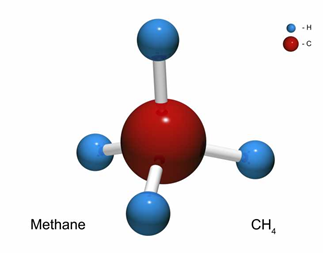
\includegraphics[scale=2]{Methane.png}

\setcounter{equation}{0}
\textbf{Solution:}\\
We will use point $A(0,0,0)$ as our first hydrogen atom, point $E\left(\frac{1}{2},\frac{1}{2},\frac{1}{2}\right)$ as our carbon atom, and $B(1,1,0)$ as our third hydrogen atom. From here, we can create two vectors, $\vec{AE}$ and $\vec{EB}$.
\begin{align}
    \vec{AE} &= \vec{E} - \vec{A} \\
    \vec{AE} &= \left(\dfrac{1}{2}, \dfrac{1}{2}, \dfrac{1}{2}\right) - (0,0,0) \\
    \vec{AE} &= \left(\dfrac{1}{2}, \dfrac{1}{2}, \dfrac{1}{2}\right)
\end{align}
\begin{align}
    \vec{EB} &= \vec{B} - \vec{E} \\
    \vec{EB} &= (1,1,0) - \left(\dfrac{1}{2}, \dfrac{1}{2}, \dfrac{1}{2}\right) \\
    \vec{EB} &= \left(\dfrac{1}{2}, \dfrac{1}{2}, -\dfrac{1}{2}\right)
\end{align}
Recall Theorem 3.2 on pg 714,
$$a\cdot b = |a||b|\cos\theta$$
Isolate $\theta$ on one side by rearranging this equation.
\begin{align}
    a\cdot b &= |a||b|\cos\theta \\
    cos\theta &= \dfrac{a \cdot b}{|a||b|} \\
    \theta &= \cos^{-1}\left(\dfrac{a \cdot b}{|a||b|}\right)
\end{align}
Sub in equivalent values for our question. We have,
$$\theta = \cos^{-1}\left(\dfrac{\vec{AE} \cdot \vec{EB}}{|\vec{AE}||\vec{EB}|}\right)$$


Determine $\vec{AE} \cdot \vec{EB}$, $|\vec{AE}|$ and $|\vec{EB}|$ separately.
\begingroup
\addtolength{\jot}{0.5em}
\begin{align}
    \vec{AE} \cdot \vec{EB} &= \left(\dfrac{1}{2}, \dfrac{1}{2}, \dfrac{1}{2}\right) \cdot \left(\dfrac{1}{2}, \dfrac{1}{2}, -\dfrac{1}{2}\right) \\
    \vec{AE} \cdot \vec{EB} &= \dfrac{1}{4}+\dfrac{1}{4}-\dfrac{1}{4} \\
    \vec{AE} \cdot \vec{EB} &= \dfrac{1}{4}
\end{align}
\endgroup
\begin{align}
    |\vec{AE}| &= \sqrt{\left(\dfrac{1}{2}\right)^2 + \left(\dfrac{1}{2}\right)^2 + \left(\dfrac{1}{2}\right)^2}\\
    |\vec{AE}| &= \sqrt{\dfrac{3}{4}}
\end{align}
\begin{align}
    |\vec{EB}| &= \sqrt{\left(\dfrac{1}{2}\right)^2 + \left(\dfrac{1}{2}\right)^2 + \left(-\dfrac{1}{2}\right)^2}\\
    |\vec{EB}| &= \sqrt{\dfrac{3}{4}}
\end{align}
Sub in all relevant values into the equation $\theta = \cos^{-1}\left(\dfrac{\vec{AE} \cdot \vec{EB}}{|\vec{AE}||\vec{EB}|}\right)$ and solve for $\theta$.
\begin{align}
    \theta &= \cos^{-1}\left(\dfrac{\vec{AE} \cdot \vec{EB}}{|\vec{AE}||\vec{EB}|}\right) \\
    \theta &= \cos^{-1}\left(\dfrac{\frac{1}{4}}{\frac{3}{4}}\right) \\
    \theta &= \cos^{-1}\left(\dfrac{1}{3}\right)\\
    \theta &\approx 70.5^{\circ}
\end{align}
However, since we have an obtuse angle, we have that,
\begin{align}
    \theta &= 180^{\circ} - 70.5^{\circ} \\
    \theta &= 109.5^{\circ}
\end{align}



\newpage

%% PROBLEM 7
\item If $\theta$ is the acute angle between $\vec{a}$ and $\vec{b}$ then prove $proj_{\vec{a}}\vec{b} \cdot proj_{\vec{b}}\vec{a} = (\vec{a} \cdot \vec{b}) \cos^2(\theta)$.\\

\textbf{Solution:}\\
Prove that the left side equals the right side,
\begingroup
\addtolength{\jot}{0.5em}
\setcounter{equation}{0}
\begin{align}
    &= proj_{\vec{a}}\vec{b} \cdot proj_{\vec{b}}\vec{a} \\
    &= \left(\dfrac{\vec{b} \cdot \vec{a}}{|\vec{a}|^2}\vec{a}\right) \cdot \left(\dfrac{\vec{a} \cdot \vec{b}}{|\vec{b}|^2}\vec{b}\right) \qquad \xleftarrow[]{\text{definition of vector projection}} \\
    &= (\vec{a} \cdot \vec{b}) \cdot \dfrac{(\vec{a} \cdot \vec{b})^2}{|\vec{a}|^2|\vec{b}|^2} \\
    &= (\vec{a} \cdot \vec{b}) \cdot \dfrac{\left(|\vec{a}||\vec{b}| \cos(\theta)\right)^2}{|\vec{a}|^2|\vec{b}|^2} \qquad \xleftarrow[]{\text{Theorem 3.2 pg. 714}}\\
    &= (\vec{a} \cdot \vec{b}) \cdot \dfrac{|\vec{a}|^2|\vec{b}|^2 \cos^2(\theta)}{|\vec{a}|^2|\vec{b}|^2} \\
    &= (\vec{a} \cdot \vec{b}) \cos^2(\theta)
\end{align}
\endgroup

\textbf{Therefore, if $\theta$ is the acute angle between $\vec{a}$ and $\vec{b}$, $$proj_{\vec{a}}\vec{b} \cdot proj_{\vec{b}}\vec{a} = (\vec{a} \cdot \vec{b}) \cos^2(\theta)$$}



\newpage

%% PROBLEM 8
\item If $\vec{a}+\vec{b}+\vec{c}=\vec{0}$ then prove $\vec{a} \times \vec{b} = \vec{b} \times \vec{c} = \vec{c} \times \vec{a}$.\\

\setcounter{equation}{0}
\textbf{Solution:}\\
Start by manipulating the given equation $\vec{a}+\vec{b}+\vec{c}=\vec{0}$.
\begin{align}
    \vec{a}+\vec{b}+\vec{c} &= \vec{0} \\
    (\vec{a}+\vec{b}+\vec{c}) \times \vec{b} &= \vec{0} \times \vec{b} \\
    \vec{a}\times\vec{b} + \vec{b}\times\vec{b} + \vec{c}\times\vec{b} &= 0 \quad \xleftarrow[]{\text{Recall } \vec{b} \times \vec{b} = 0}\\
    \vec{a}\times\vec{b} + \vec{c}\times\vec{b} &= 0 \\
    \vec{a}\times\vec{b} &= -(\vec{c}\times\vec{b})
\end{align}
Recall Theorem 4.3 on pg. 726, for some $\vec{a},\vec{b}$, we have that $\vec{a}\times\vec{b} = -(\vec{a}\times\vec{b})$, or, that the cross product operation is anti-commutative. By the anti-commutative law of the cross product, we have that
$$-(\vec{c}\times\vec{b}) = \vec{b}\times\vec{c}$$
Therefore, we can express line (5) as follows,
\begin{align}
    \vec{a}\times\vec{b} &= -(\vec{c}\times\vec{b}) \\
    \vec{a}\times\vec{b} &= \vec{b}\times\vec{c}
\end{align}
Now, repeat the same process, this time manipulating the given equation $\vec{a}+\vec{b}+\vec{c}=\vec{0}$ by multiplying both sides by $\vec{c}$.
\begin{align}
    \vec{a}+\vec{b}+\vec{c} &= \vec{0} \\
    (\vec{a}+\vec{b}+\vec{c}) \times \vec{c} &= \vec{0} \times \vec{c} \\
    \vec{a}\times\vec{c} + \vec{b}\times\vec{c} + \vec{c}\times\vec{c} &= 0 \\
    \vec{a}\times\vec{c} + \vec{b}\times\vec{c} &= 0 \\
    \vec{b}\times\vec{c} &= -(\vec{a}\times\vec{c}) \\
    \vec{b}\times\vec{c} &= \vec{c}\times\vec{a}
\end{align}
Since $\vec{a}\times\vec{b} = \vec{b}\times\vec{c}$ and $\vec{b}\times\vec{c} = \vec{c}\times\vec{a}$. We have that, $$\vec{a}\times\vec{b} = \vec{b}\times\vec{c} = \vec{c}\times\vec{a}$$\\

\textbf{Therefore, if $\vec{a}+\vec{b}+\vec{c}=\vec{0}$, we have that $\vec{a}\times\vec{b} = \vec{b}\times\vec{c} = \vec{c}\times\vec{a}$}


\newpage

%% PROBLEM 9
\item Determine the equation of a line through the point $A(1,2,-3)$ and lying within the plane $x-2y+2z+9=0$.\\

\textbf{Solution:}\\
Consider some point $B(-9,0,0)$, verify that this point lies within the plane $x-2y+2z+9=0$.\\
\setcounter{equation}{0}
\begin{align}
    0 &= x-2y+2z+9 \\
    0 &= (-9)-2(0)+2(0)+9 \\
    0 &= 0
\end{align}
Since the equation above is true, I have verified that point $B$ lies within the plane $x-2y+2z+9=0$.

Determine an equation of a line that passes through $(1,2,-3)$ and $(-9,0,0)$. Let's start with the vector form, we have,
$$\vec{r} = (1,2,-3) + t(a,b,c)$$
Determine the direction vector by subtracting point A from point B,
\begin{align}
    (a,b,c) &= (-9-1,0-2,0-(-3))\\
    (a,b,c) &= (-10,-2,3)
\end{align}
We have that the equation of the line from $A$ to $B$ is $$\vec{r} = (1,2,-3) + t(-10,-2,3)$$
Since this line goes through $A$ and $B$, and $A$ and $B$ are both on the plane $x-2y+2z+9=0$, we have that the line $\vec{r} = (1,2,-3) + t(-10,-2,3)$ also lies on the plane $x-2y+2z+9=0$.\\

\textbf{Therefore, one possible equation of a line, in vector form, that goes through point $A(1,2,-3)$ and lies within the plane $x-2y+2z+9=0$ is $$\vec{r} = (1,2,-3) + t(-10,-2,3)$$}

\newpage

%% PROBLEM 10
\item Determine the equation of a plane through the origin and the points $P(3,1,2)$ and $Q(-1,2,-3)$.\\

\textbf{Solution:}\\

\textbf{Vector Form}\\
First, we need to determine the direction vectors of this plane by selecting two pairs of non-zero, non-collinear vectors from the given points, $O,P,Q$.\\
Let's use $\vec{OP}$ and $\vec{OQ}$, we have,
\setcounter{equation}{0}
\begin{align}
    \vec{OP} &= (3-0,1-0,2-0) \\
    \vec{OP} &= (3,1,2) \\
    \vec{OQ} &= (-1-0,2-0,-3-0) \\
    \vec{OQ} &= (-1,2,-3)
\end{align}
Now that we have the direction vectors for this plane, we can determine the position vector. \\
Let's choose point $P(3,1,2)$ to be our position vector. We have that the equation of this plane in Vector Form is,
$$\vec{r} = s(3,1,2)+t(-1,2,-3)+(3,1,2)$$

\textbf{Cartesian Form}\\
Determine the normal vectors,
\begin{align}
    \vec{n} &=
    \begin{pmatrix}
       \vec{i} & \vec{j} & \vec{k} \\
       3 & 1 & 2 \\
       -1 & 2 & -3
    \end{pmatrix}\\
    \vec{n} &= -7\vec{i} + 7\vec{j} + 7\vec{k}
\end{align}
From the normal vectors, we can sub in the corresponding coefficients of $\vec{i}, \vec{j}, \vec{k}$ into the cartesian form, $Ax+By+Cz+D=0$. We have,
$$-7x+7y+7z+D=0$$
I can determine $D$ by subbing in the coordinates of the origin, $(0,0,0)$ into $(x,y,z)$. By inspection, I can determine that $D=0$. Therefore, the equation of the plane going through points $O,P,Q$ in Cartesian Form is,
$$-7x+7y+7z=0$$

\textbf{Therefore, the equation of the plane that goes through the origin, the points $P(3,1,2)$ and $Q(-1,2,-3)$, is
$$\vec{r} = s(3,1,2)+t(-1,2,-3)+(3,1,2)$$
or
$$-7x+7y+7z=0$$}


\newpage


%% PROBLEM 11
\item Determine the (\emph{least}) distance between the point $A(1,-2,4)$ and the plane $3x+2y+6z-5=0$.

\newpage

\setcounter{equation}{0}
%% PROBLEM 12
\item Suppose that $\vec{v_1}$ and $\vec{v_2}$ are vectors such that $|\vec{v_1}|=2$ and $|\vec{v_2}| = 3$, and $\vec{v_1} \cdot \vec{v_2} = 5	$. Let $\vec{v_3} = proj_{\vec{v_1}}\vec{v_2}$, $\vec{v_4} = proj_{\vec{v_2}}\vec{v_3}$ and so on so that $\vec{v_{k+1}} = proj_{\vec{v_{k-1}}}\vec{v_k}$.  Evaluate $\sum\limits_{i=1}^{\infty} |\vec{v_i}|$.\\

\textbf{Solution:}\\
By definition, we have that,
\begin{align}
    \sum\limits_{i=1}^{\infty} |\vec{v_i}| &= |\vec{v_1}| + |\vec{v_2}| + |\vec{v_3}| + ... + |\vec{v_{\infty-1}}| + |\vec{v_\infty}| + ...
\end{align}
Recall the magnitude of some $proj_{\vec{b}}\vec{a}$ is $$comp_{\vec{b}}\vec{a} = \dfrac{\vec{a} \cdot \vec{b}}{|\vec{b}|}$$
Since $\vec{v_{k+1}} = proj_{\vec{v_{k-1}}}\vec{v_k}$, we have that $$|\vec{v_{k+1}}| = \dfrac{\vec{v_k} \cdot \vec{v_{k-1}}}{|\vec{v_{k-1}}|}$$
Therefore, we have that,
\begin{align}
    \sum\limits_{i=1}^{\infty} |\vec{v_i}| &= |\vec{v_1}| + |\vec{v_2}| + |\vec{v_3}| + ... + |\vec{v_{\infty-1}}| + |\vec{v_\infty}| + ... \\
    \sum\limits_{i=1}^{\infty} |\vec{v_i}| &= 2 + 3 + \dfrac{\vec{v_2} \cdot \vec{v_{1}}}{|\vec{v_{1}}|} + \dfrac{\vec{v_3} \cdot \vec{v_{2}}}{|\vec{v_{2}}|} + \dfrac{\vec{v_4} \cdot \vec{v_{3}}}{|\vec{v_{3}}|} + ... \\
    \sum\limits_{i=1}^{\infty} |\vec{v_i}| &= 2 + 3 + \dfrac{|\vec{v_2}||\vec{v_1}|\cos\theta}{|\vec{v_{1}}|} + \dfrac{|\vec{v_3}||\vec{v_2}|\cos\theta}{|\vec{v_{2}}|} + \dfrac{|\vec{v_4}||\vec{v_3}|\cos\theta}{|\vec{v_{3}}|} + ... \quad \xleftarrow[]{\text{Theorem 3.2 pg. 714}} \\
    \sum\limits_{i=1}^{\infty} |\vec{v_i}| &= 2 + 3 + |\vec{v_2}|\cos\theta + |\vec{v_3}|\cos\theta + |\vec{v_4}|\cos\theta + ...
\end{align}
Let's take a closer look at line (5), specifically the individual terms on the right hand side of the equation,
$$\sum\limits_{i=1}^{\infty} |\vec{v_i}| = \underbrace{2}_{|v_1|} + \underbrace{3}_{|v_2|} + \underbrace{|\vec{v_2}|\cos\theta}_{|v_3|} +  \underbrace{|\vec{v_3}|\cos\theta}_{|v_4|} + | \underbrace{|\vec{v_4}|\cos\theta}_{|v_5|} + ...$$

Notice how $|\vec{v_3}|$ is defined by $|\vec{v_2}|$, $|\vec{v_4}|$ is defined by $|\vec{v_3}|$, $|\vec{v_5}|$ is defined by $|\vec{v_4}|$ and so forth. We can re-define $|\vec{v_3}|, |\vec{v_4}|, |\vec{v_5}|,... $ such that they are all defined by $|\vec{v_2}|$,
\begingroup
\addtolength{\jot}{0.8em}
\begin{align}
    |\vec{v_2}| &= |\vec{v_2}| \\
    |\vec{v_3}| &= |\vec{v_2}|\cos\theta \\
    |\vec{v_4}| &= \underbrace{\left(|\vec{v_2}|\cos\theta\right)}_{|\vec{v_3}|}\cos\theta \\
    |\vec{v_5}| &= \underbrace{\left(\underbrace{\left(|\vec{v_2}|\cos\theta\right)}_{|\vec{v_3}|}\cos\theta\right)}_{|\vec{v_4}|}\cos\theta
\end{align}
\endgroup

With this, let's rewrite line (5),
\begin{align}
    \sum\limits_{i=1}^{\infty} |\vec{v_i}| &= 2 + |\vec{v_2}| + |\vec{v_2}|\cos\theta + |\vec{v_2}|\cos\theta\cos\theta + |\vec{v_2}|\cos\theta\cos\theta\cos\theta + ... \\
    \sum\limits_{i=1}^{\infty} |\vec{v_i}| &= 2 + |\vec{v_2}| + |\vec{v_2}|\cos\theta + |\vec{v_2}|\cos^2\theta + |\vec{v_2}|\cos^3\theta + ... \\
    \sum\limits_{i=1}^{\infty} |\vec{v_i}| &= 2 + |\vec{v_2}| \left(\cos\theta + \cos^2\theta + \cos^3\theta + ... \right) \\
    \sum\limits_{i=1}^{\infty} |\vec{v_i}| &= 2 + |\vec{v_2}| \sum\limits_{i=0}^{\infty}\left(\cos^i(\theta)\right) \\
    \sum\limits_{i=1}^{\infty} |\vec{v_i}| &= 2 + 3 \sum\limits_{i=0}^{\infty}\left(\cos^i(\theta)\right) \qquad \qquad \xleftarrow[]{|\vec{v_2}| \,=\, 3}
\end{align}
Recall that for some $\vec{v_1}, \vec{v_2}$, we have that
\begingroup
\addtolength{\jot}{0.5em}
\begin{align}
    \vec{v_1}\cdot\vec{v_2} &= |\vec{v_1}||\vec{v_2}|\cos\theta \\
    \cos\theta &= \dfrac{\vec{v_1} \cdot \vec{v_2}}{|\vec{v_1}||\vec{v_2}|} \\
    \cos\theta &= \dfrac{(5)}{(2)(3)} \qquad \xleftarrow[]{\text{values given from the question}} \\
    \cos\theta &= \dfrac{5}{6}
\end{align}
\endgroup
Now that we know that $\cos\theta = \dfrac{5}{6}$, we can sub this into line (14),
\begin{align}
    \sum\limits_{i=1}^{\infty} |\vec{v_i}| &= 2 + 3 \sum\limits_{i=0}^{\infty}\left(\dfrac{5}{6}\right)^i
\end{align}
Recall that the sum of a geometric series is,
$\sum\limits_{i=0}^{n}r^i = \dfrac{1-r^n}{1-r}$\\
Let $r=\dfrac{5}{6}$, $n=\infty$, we have that,
\begin{align}
    \sum\limits_{i=1}^{\infty} |\vec{v_i}| &= 2 + 3 \sum\limits_{i=0}^{\infty}\left(\dfrac{5}{6}\right)^i \\
    \sum\limits_{i=1}^{\infty} |\vec{v_i}| &= 2 + 3 \left(\dfrac{1-\left(\frac{5}{6}\right)^n \xleftarrow[]{\text{approaches 0}}}{1-\left(\frac{5}{6}\right)}\right)\\
    \sum\limits_{i=1}^{\infty} |\vec{v_i}| &= 2 + 3 \left(\dfrac{1}{1-\left(\frac{5}{6}\right)}\right)\\
    \sum\limits_{i=1}^{\infty} |\vec{v_i}| &= 20
\end{align}
$$\therefore \sum\limits_{i=1}^{\infty} |\vec{v_i}| = 20$$



\newpage

%% PROBLEM 13
\item Determine and classify the nature of the intersection between the following planes:
$$\Pi_1: x-5y+2z=10 $$
$$\Pi_2: x+7y-2z+6=0 $$
$$\Pi_3: 8x+5y+z=20 $$


\LaTeX{} note: You may find the \emph{amatrix} custom environment included in the code useful for creating the augmented matrix below.\\

$
\begin{amatrix}{3}
   1 & -5 & 2 & 10\\  1 & 7 & -2  & -6\\ 8 & 5 & 1 & 20 
 \end{amatrix}
$\\

%% $\equiv$ gives the "triple equal sign" equivalence relation if you want to use that for row equivalent matrices 

\textbf{Solution:}\\
By inspection, I can see that the three planes have non-collinear normal vectors. Since they have non-collinear normals, we can determine the nature of the intersection by creating an augmented matrix system and reducing it in Row Echelon Form(REF).
\setcounter{equation}{0}
\begingroup
\addtolength{\jot}{0.5em}
\begin{align}
    &\begin{amatrix}{3}
        1 & -5 & 2 & 10\\
        1 & 7 & -2  & -6\\
        8 & 5 & 1 & 20 
    \end{amatrix}\\
    \equiv
    \substack{{R_2}^{'} =\, R_1-R_2 \\
    {R_3}^{'} =\, 8R_1-R_3}
    &\begin{amatrix}{3}
       1 & -5 & 2 & 10\\
       0 & -12 & 4  & 16\\
       0 & -45 & 15 & 60 
    \end{amatrix}\\
    \equiv
    {R_2}^{'} =\, \dfrac{1}{12}R_2
    &\begin{amatrix}{3}
       1 & -5 & 2 & 10\\
       0 & -1 & \frac{1}{3}  & \frac{4}{3}\\
       0 & -45 & 15 & 60 
    \end{amatrix}\\
    \equiv
    {R_3}^{'} =\, 45R_2-R_3
    &\begin{amatrix}{3}
       1 & -5 & 2 & 10\\
       0 & -1 & \frac{1}{3}  & \frac{4}{3}\\
       0 & 0 & 0 & 0
    \end{amatrix}
\end{align}
\endgroup
We have a tautology case in the third row of line (4), therefore, $z$ is a \textit{free variable} and any value of $z$ will satisfy $R_3$. So, we will need to parameterize this variable.

Let $z = t \quad (t \in \mathbb{R})$\\

From $R_2$, we have,
\begingroup
\addtolength{\jot}{0.5em}
\begin{align}
    -1y + \dfrac{1}{3}z &= \dfrac{4}{3}\\
    -y + \dfrac{1}{3}t &= \dfrac{4}{3} \quad \xleftarrow[]{z\,=\, t}\\
    y &= \dfrac{1}{3}t-\dfrac{4}{3}
\end{align}
\endgroup
From $R_1$, we have,
\begingroup
\addtolength{\jot}{0.5em}
\begin{align}
    1x -5y + 2z &= 10 \\
    x &= 10 - 2z + 5y \\
    x &= 10 - 2t + 5\left(\dfrac{1}{3}t-\dfrac{4}{3}\right) \quad \xleftarrow[]{z \, = \, t \text{ and } y \, = \, \frac{1}{3}t-\frac{4}{3}}\\
    x &= 10 -2t + \dfrac{5}{3}t - \dfrac{20}{3} \\
    x &= -\dfrac{1}{3}t + \dfrac{10}{3}
\end{align}
\endgroup
Therefore, the solution to this system is
$$(x,y,z) = \left(-\dfrac{1}{3}t + \dfrac{10}{3},\, \dfrac{1}{3}t-\dfrac{4}{3},\, t\right) \qquad \qquad \qquad (t \in \mathbb{R})$$
We can also express the solution as a line in vector form.
\begin{align}
    \vec{r} &= t\vec{d} + \vec{r}_0 \\
    \vec{r} &= t\left(-\dfrac{1}{3}, \dfrac{1}{3}, 1\right) + \left(\dfrac{10}{3},-\dfrac{4}{3},0\right)
\end{align}

Since the three planes are consistent and:

\begin{minipage}{0.5\textwidth}
    \begin{itemize}
        \item Have infinite solutions in a linear systems
        \item Intersect along a line
        \item Do not have collinear normal vectors
        \item Required variable parameterization
    \end{itemize}
\end{minipage}
\begin{minipage}{0.5\textwidth}
    \begin{figure}[H]
    \centering{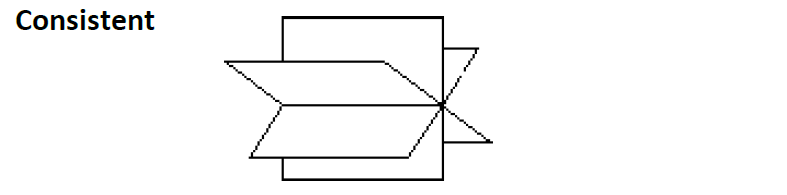
\includegraphics[width=9cm]{Q13Image.png}}
    \caption{Nature of intersection of three planes}
    \end{figure} 
\end{minipage}\\\\

\textbf{$\therefore \quad \Pi_1,\Pi_2$ and $\Pi_3$ intersect along a line and are non-coincident planes (Figure 1).}



\newpage

\setcounter{equation}{0}
%% PROBLEM 14
\item Given $A=\bigg(\begin{smallmatrix} -1 & \frac{3}{2} \\ 1 & -1 \\ \end{smallmatrix}\bigg)$, demonstrate that $det(A) \neq 0$ which implies that $A^{-1}$ exists. Then, determine $A^{-1}$ and verify $AA^{-1} = I$.\\

\textbf{Solution:}\\
Begin by demonstrating that $A=\bigg(\begin{smallmatrix} -1 & \frac{3}{2} \\ 1 & -1 \\ \end{smallmatrix}\bigg)$ does indeed have an inverse matrix, $A^{-1}$.\\ Determine $det(A)$.
\begin{align}
    A &= \bigg(\begin{smallmatrix}
    -1 & \frac{3}{2} \\
    1 & -1 \\
    \end{smallmatrix}\bigg)\\
    det(A) &= (-1)(-1) - (1)\left(\dfrac{3}{2}\right) \\
    det(A) &= -\dfrac{1}{2}
\end{align}
\textbf{Therefore, the inverse matrix, $A^{-1}$ exists because $det(A) \neq 0$.}\\

Now we can determine $A^{-1}$. Consider some 2x2 matrix $N = \bigg(\begin{smallmatrix} a & b \\ c & d \\ \end{smallmatrix}\bigg)$, recall that its inverse matrix, $N^{-1}$ is,
$$N^{-1} = \dfrac{1}{det(N)} \bigg(\begin{smallmatrix} d & -b \\ -c & a \\ \end{smallmatrix}\bigg)$$
By the same token, we have that $A^{-1}$ is,
\begingroup
\addtolength{\jot}{0.5em}
\begin{align}
    A^{-1} &= \dfrac{1}{det(A)} \bigg(\begin{smallmatrix} -1 & -\frac{3}{2} \\ -1 & -1 \\ \end{smallmatrix}\bigg) \\
    A^{-1} &= \dfrac{1}{-\frac{1}{2}} \bigg(\begin{smallmatrix} -1 & -\frac{3}{2} \\ -1 & -1 \\ \end{smallmatrix}\bigg) \\
    A^{-1} &= -2 \bigg(\begin{smallmatrix} -1 & -\frac{3}{2} \\ -1 & -1 \\ \end{smallmatrix}\bigg) \\
    A^{-1} &= \bigg(\begin{smallmatrix} 2 & 3 \\ 2 & 2 \\ \end{smallmatrix}\bigg)
\end{align}
\endgroup
\textbf{Therefore, we have that $A^{-1} = \bigg(\begin{smallmatrix} 2 & 3 \\ 2 & 2 \\ \end{smallmatrix}\bigg)$}\\

Verify that $AA^{-1} = I$. Consider some matrix $P = \bigg(\begin{smallmatrix} a & b \\ c & d \\ \end{smallmatrix}\bigg)$ and some matrix $Q = \bigg(\begin{smallmatrix} x & y \\ z & k \\ \end{smallmatrix}\bigg)$, the product of $P$ and $Q$ is $PQ = \bigg(\begin{smallmatrix} ax+bz & ay+bk \\ cx+dz & cy+dk \\ \end{smallmatrix}\bigg)$. By the same token, we have that,
\begingroup
\addtolength{\jot}{0.5em}
\begin{align}
    AA^{-1} &= \bigg(\begin{smallmatrix} -1 & \frac{3}{2} \\ 1 & -1 \\ \end{smallmatrix}\bigg) \bigg(\begin{smallmatrix} 2 & 3 \\ 2 & 2 \\ \end{smallmatrix}\bigg) \\
    AA^{-1} &= \bigg(\begin{smallmatrix} (-1)(2)+\left(\frac{3}{2}\right)(2) & (-1)(3)+\left(\frac{3}{2}\right)(2) \\ (1)(2)+(-1)(2) & (1)(3)+(-1)(2) \\ \end{smallmatrix}\bigg) \\
    AA^{-1} &= \bigg(\begin{smallmatrix} 1 & 0 \\ 0 & 1 \\ \end{smallmatrix}\bigg)
\end{align}
\endgroup
\textbf{Therefore, the product of $A$ and its inverse equals the identity matrix, $AA^{-1} = I$.}

\newpage

\begin{center}
    
    \centering\large{Therefore, I have finished MCV4UR.}\\
    
    Thank you for being a great Grade 11 and Grade 12 Math teacher, Mr. Blakely!\\
    Have a great summer!\\
    \textbf{QED}\\
\end{center}

\centering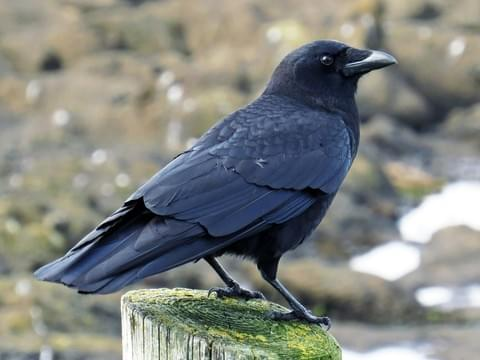
\includegraphics[scale=0.8]{Question2020Image.jpg}



\end{enumerate}
\end{document} 
